 \documentclass[12pt]{article}
\usepackage[spanish, mexico]{babel} % espanol
\usepackage[utf8]{inputenc} % acentos sin codigo
\usepackage{enumerate} % enumerados
\usepackage{amsmath}
\usepackage{amsfonts}
\usepackage{amssymb}
\usepackage{graphicx}
\usepackage{float}

\title{Actividad 5}
\author{Paulina Valenzuela Coronado}
\date{Enero 2016}
\begin{document}
\maketitle

\section{El Péndulo}

Un péndulo simple está constituido por un hilo inextensible de masa despreciable, sostenido por su extremo superior de un punto fijo, con una masa puntual sujeta en su extremo inferior que oscila libremente en un plano vertical fijo.
El movimiento solo ocurre en dos dimensiones y este no pierde energía por la fricción o la resistencia del aire.\cite{Wiki} \\

La ecuación del movimiento de un péndulo simple es 

\begin{equation}
\frac{
d^2\theta}{dt^2}+\frac{g}{l}\sin\theta=0
\end{equation}

donde
\begin{itemize}
\item $g$ es la aceleración debida a la gravedad
\item $l$ es el lago del péndulo
\item $\theta$ es el desplazamiento angular 
\end{itemize}

\begin{figure}[H]
	\centering
\includegraphics[width=5cm]{12.png}
 \caption{Péndulo simple}
\end{figure} 

Para resolver la ecuación 1 se requiere del uso de métodos númericos, en esta actividad se pide describir el problema del péndulo, sus ecuaciones de movimiento y la forma de resolverlas numéricamente utilizando la funcion \textit{scipy.integrate.odeint} de Python.
Esta herramienta integra sistemas de ecuaciones diferenciales ordinarias, resuele el sistema utilizando la herramienta "Isoda" de la librería de FORTRAN.
Resuelve el problema del valor inicial en sistemas rígidos o no rígidos de primer orden. \\

\textbf{Programa:}
La ecuación diferencial de segundo orden 
para un ángulo $\theta$ de un péndulo actuando debido a la gravedad y a la fricción puede escribirse como:

$$\theta''(t)+b*\theta'(t)+c*\sin(\theta(t))=0$$
donde $b$ y $c$ son constantes positivas.
Para resolver esta ecuación tenemos que convertir en un sistema de ecuaciones de primer orden. Para definir la velocidad angular
$\omega(t)=\theta'$, tenemos el siguiente sistema:
$$\theta'(t) = \omega(t)
\omega'(t) = -b*\omega(t) - c*\sin(\theta(t))$$
Dejando $y$ como el vector $[\theta, \omega]$. A continuación se muestra el código completo y una serie de ejemplos en los que se cambian las condiciones iniciales para poder simular y entender mejor estos movimientos.

\begin{verbatim}
def pend(y, t, b, c):
theta, omega = y
dydt = [omega, -b*omega - c*np.sin(theta)]
return dydt

b = 0
c = 0.5


y0 = [np.pi - 0.2, 0.0]

t = np.linspace(0, 100, 101)



from scipy.integrate import odeint
sol = odeint(pend, y0, t, args=(b, c))


import matplotlib.pyplot as plt
plt.plot(t, sol[:, 0], 'b', label='theta(t)')
plt.plot(t, sol[:, 1], 'g', label='omega(t)')
plt.legend(loc='best')
plt.xlabel('t')
plt.grid()
plt.show()
\end{verbatim}


\begin{figure}[H]
	\centering
\includegraphics[width=8cm]{1.jpg}	
\caption{$\theta=\pi - 0.1$}
\end{figure}

\begin{figure}[H]
	\centering
	\includegraphics[width=8cm]{2.jpg}	
	\caption{$\theta=\pi - 0.36$}
\end{figure}

\begin{figure}[H]
	\centering
	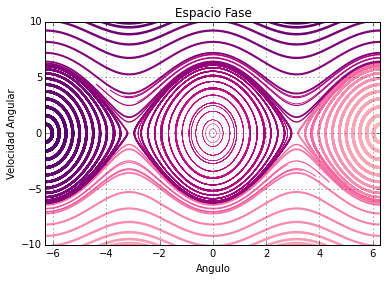
\includegraphics[width=8cm]{3.jpg}	
	\caption{$\theta=\pi - 0.5$}
\end{figure}


\begin{thebibliography}{9}
	
	\bibitem{Wiki}
Wikipedia en Español, https://es.wikipedia.org/wiki/P%C3%A9ndulo
	\emph{Péndulo}
	
		
\end{thebibliography}



\end{document}